\section{Resource allocation for a system following a pipe and filter like architecture}
This section focuses on the main challenges of implementing resource allocation without losing fault tolerance or decoupling between components. Replicas of the same component have no means of organizing, they just take the next job that is available in the queue and execute it, no mechanism for distributing the jobs is in place. Replicas of the same component can consume different amounts of system resources, depending on the type of job they are executing, bat because they have no possibility to select the jobs they will execute, they just take the next job from the queue, we cannot predict on which of the replicas the job will be executed. Because of this unpredictability, the task of allocating resources becomes challenging and different methods have been proposed.

Replicas for the "Scanner" component were used as a case study and the following strategies were considered. Jobs present in the queue were marked as H, M, L denoting the CPU usage necessary in order to complete that particular job.


\subsection{Method 1: Allows the system to balance work in a natural way and not intervene in job allocation}
The first strategy was to let the replicas of the "Scanner" component execute whatever job is available in the queue if they are idle. The main advantages of this strategy is that it does not require any changes to the system, so no extra complexity is added. Fig. \ref{fig:randomDIstributionsOfTasks} presents the architecture of the first approach. Another advantage is that components are decoupled as envisioned in the initial architecture Fig. \ref{fig:systemArchitecture}.

The main drawback of this approach is that, because balancing is done by change, in the worst case, the system could be completely unbalanced, some component executing only high intensive CPU jobs while others executing only low CPU intensive jobs. If more than one "Scanner" replicas run on the same VM, than the chances are even lower for this to happen because, even if some component would bu "unlucky" enough to only execute CPU intensive jobs, they would be balanced by other components that execute low intensive CPU jobs from the same machine.

\begin{figure}[ht]
\centering
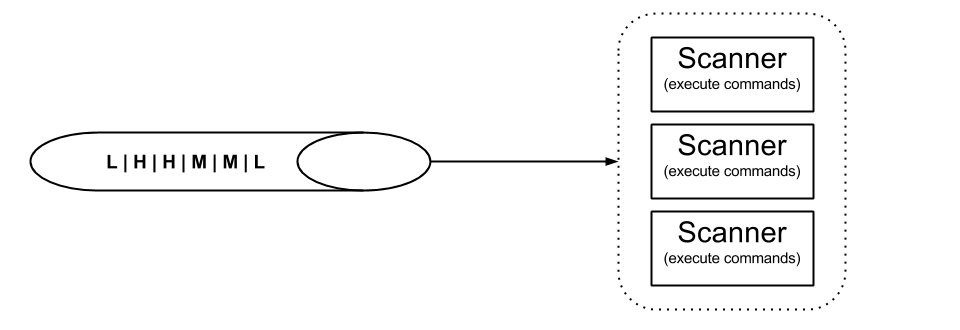
\includegraphics[width=\linewidth]{./img/1_NaturalLoadBalancing.png}
\caption{Random distribution of tasks}
\label{fig:randomDIstributionsOfTasks}
\end{figure}

\subsection{Method 2: Assign sizes to jobs and constrain component replicas to execute some type of jobs with a higher priority than others}
The second approach proposes using some priority scheme inside the "Scanner" component replicas so that we can place "Scanner" replicas on machines that satisfy the computational needs that are required. For example if we have a machine with more CPU power, we can allocate "Scanner" replicas that execute CPU intensive jobs. The main advantage of this approach is that we can allocate Scanner replicas with different priority schemes to different types of VM's, obtaining a coordinated assignment of jobs. 

Because we use the message queue, and every component need to withdraw one message from the queue in order to inspect it, if the "Scanner" replica withdraws a message that does not fit it's priority scheme, it must put the message in the front of the queue. Because of this, some messages may spend a very long time in the queue, or even never get executed, if they are always delivered to components that cannot handle them and are put back in the front of the queue.Another problem is that the queue is more stressed, because messages are inserted back in the queue if they cannot be executed by a "Scanner" replicas.


Fig. \ref{fig:sizeBaseDistributionOftasks}

\begin{figure}[ht]
\centering
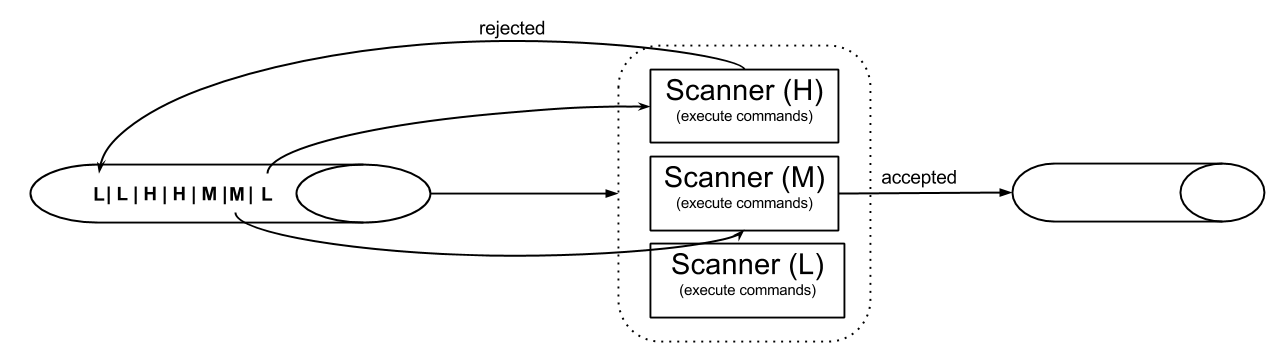
\includegraphics[width=\linewidth]{./img/2_PriorityLoadBalancing.png}
\caption{Size base distribution of tasks}
\label{fig:sizeBaseDistributionOftasks}
\end{figure}



\subsection{Method 3: Create multiple queues deepening on the size of the jobs}

\subsection{Method 4: Use other types of data structure to send the jobs from one component to another}


\subsection{Choosing one method}
One of the assumption made at the beginning of this section was that we can determine in advance the CPU usage for jobs, but this can prove to be very difficult in practice because there are more than 3 types of jobs and they CPU usage depends on other factors like network speed and the speed of response for a particular host, network configuration, etc.

As a starting point we chose method 1 (reference to subsection 1) because it does not break any of the properties the system has, it can be later extended to any of the more advanced methods and in practice we observed that "Scanner" replicas tend to balanced themselves naturally, without any intervention.